\begin{sepframe}{Complexity}
    {\scriptsize{Simplicity is the ultimate sophistication. L. Da Vinci}}
\end{sepframe}

\begin{frame}
    \frametitle{Complexity}
    \framesubtitle{Complexity at a glance}

    \begin{itemize}[<+->]
        \item Used to compare algorithms efficiency,
        \item Often calculated using the worst case scenario (usually \textit{when the input grow infinitely})
        \item In ``Big $\mathcal{O}$'' notation: $\mathcal{O}(1)$, $\mathcal{O}(n)$, $\mathcal{O}(n \times log(n))$, $\mathcal{O}(n^2)$
    \end{itemize}

    \note[item]{
        Let's make a reminder on what complexity is.
    }

    \note[item]{
        Read the bullet points
    }
\end{frame}

\begin{frame}
    \frametitle{Complexity}
    \framesubtitle{Types}

    \begin{itemize}[<+->]
        \item Time complexity
        \item Space complexity
        \item Kolmogorov complexity
        \item Cyclomatic complexity
    \end{itemize}

    \note[item]{
        How about now diving into the marvellous world of algorithmic
        complexity?
        Worry not! We are just going to scratch the surface, nothing fancy
        at all.
    }
    \note[item]{
        We are going to "explore" 4 complexity types. Here they are.
    }
    \note[item]{
        Lets start with the first one, this is usually the most classical one
        when dealing with algorithms.
    }
\end{frame}

\begin{frame}
    \frametitle{Complexity}
    \framesubtitle{Constant time complexity: $\mathcal{O}(1)$}
    \lstinputlisting{src/session/complexity/resources/time-complexity-constant.php}

    \note[item]{
        Let's explain the time complexity with some examples...
    }
    \note[item]{
        Here's the first one. Can you guess what this snippet is doing?
    }
    \note[item]{
        Well, here's the solution. This snippet is returning the first item
        of any type of iterable. If we had to measure its complexity, it would
        be $\mathcal{O}(1)$
    }
    \note[item]{
        Pay attention, here we are not measuring the time, we are measuring how
        much unit of time on a particular computer, no matter how fast or slow
        it is, it would take to get the
        expected output when the size of the input grows infinitely.
    }
\end{frame}

\begin{frame}
    \frametitle{Complexity}
    \framesubtitle{Linear time complexity: $\mathcal{O}(n)$}
    \lstinputlisting{src/session/complexity/resources/time-complexity-linear.php}
    \note[item]{
        Just by looking at it, can you guess what this algo is doing?
    }
    \note[item]{
        Well, here's the solution. This snippet is returning the first item
        of any type of iterable.
        The algorithm must go through each single one item of the iterable,
        therefore, $\mathcal{O}(n)$ is the complexity.
    }
\end{frame}

\begin{frame}
    \frametitle{Complexity}
    \framesubtitle{Exponential time complexity: $\mathcal{O}(n^2)$}
    \lstinputlisting{src/session/complexity/resources/time-complexity-exp.php}
    \note[item]{
        This algorithm is a bit different, it contains nested loops...
    }
    \note[item]{
        Well, here's the solution. This snippet is returning the sum of all
        items in the matrix.
        The algorithm must go through each single row then each single column,
        therefore, $\mathcal{O}(n^2)$ is the complexity.
    }
\end{frame}

\begin{frame}
    \frametitle{Complexity}
    \framesubtitle{Space complexity}
    \lstinputlisting{src/session/complexity/resources/space-complexity.php}

    \note[item]{
        Let's no focus on the algorithm here. We see that a variable \$data is
        is an array of n elements. We also see that the variable \$sum holds
        one element. Therefore the complexity if $\mathcal{O}(n + 1)$, and then
        when n goes up to infinity, $\mathcal{O}(n)$.
    }
\end{frame}

\begin{frame}
    \frametitle{Complexity}
    \framesubtitle{Kolmogorov complexity}

    The Kolmogorov complexity is the shortest size of a program that yield the
    expected output.

    \note[item]{
        The Kolmogorov complexity, besides its funny name, is something not so
        common in our day to day development.
    }
    \note[item]{
        I wanted to talk about it because I want to show that there are different
        types of complexity but also this might be something you already
        encountered without even knowing that it has a name.
    }
    \note[item]{
        I'm going to explain it by showing an example here under.
    }
\end{frame}

\begin{frame}
    \frametitle{Complexity}
    \framesubtitle{Kolmogorov complexity}

    \begin{scriptsize}
        \begin{itemize}[<+->]
            \item \texttt{1111111111111111111111111111111111111111111111111111111111111111}
            \item \texttt{317b773017df0ab62b15cd3f2ad17d7b13ab02f05f4943011ef8c4067d1ca0a5}
        \end{itemize}
    \end{scriptsize}

    \note[item]{
        Here are two strings of 64 characters each.
    }
    \note[item]{
        Can you guess which one of these strings has the smallest algorithm
        yielding those strings?
    }
    \note[item]{
        Another way to do this, let's say that you're on the phone with your
        friend. Your phone is running out of battery and could shut down at any
        moment. Which one of these strings would be faster and easier to
        describe to your friend so he can write it down?
    }
\end{frame}

\begin{frame}
    \frametitle{Complexity}
    \framesubtitle{Kolmogorov complexity}

    \lstinputlisting{src/session/complexity/resources/kolmogorov-complexity-example1.php}
\end{frame}

\begin{frame}[fragile,c]
    \frametitle{Complexity}
    \framesubtitle{Kolmogorov complexity}

    \makebox[\linewidth]{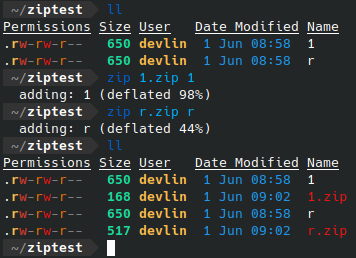
\includegraphics[height=.70\paperheight]{src/session/complexity/resources/Screenshot_20220601_090230.png}}
\end{frame}

\begin{frame}
    \frametitle{Complexity}
    \framesubtitle{Kolmogorov complexity}
    \begin{itquote}
        There is no way to tell if the Kolmogorov complexity of an algorithm is
        the shortest one.
    \end{itquote}

    \note[item]{
        The Kolmogorov complexity is the generalization of Shannon's theory of
        information.
    }
    \note[item]{
        It has links to many other fields like with Gödel's incompleteness
        theorem, Turing's halting problem, compression theory, ...
    }

    \note[item]{
        There is no mechanical device to determine the size of the smallest
        program that produces a given string. It is not that our current level
        of computer technology is insufficient for the task at hand, or that we
        are not clever enough to write the algorithm. Rather, it was proven that
        the very notion of description and computation shows that no such
        computer can ever possibly perform the task for every string. While a
        computer might find some pattern in a string, it cannot find the best
        pattern. We might find some short program that outputs a certain
        pattern, but there could exist an even shorter program. We will never
        know.
    }
    \note[item]{
        The proof that the Kolmogorov complexity of a sequence is not computable
        is a bit technical. But it is a proof by contradiction, and we can get a
        sense of how that works by looking at a paradoxe.
        We can prove that a computer will never be able to find the best pattern
        with this little story...
        Let's say we look at naturals numbers and we claim that every single
        natural have interesting properties.
        1 because it's the first number.
        2 because it's the first even number.
        3 because it's the first odd number.
        4 because it's 2+2 or 2x2...
        We can continue very far. At some point let's say we come to a number
        that does not have interesting properties and call it
        "first uninteresting number". But that in itself, is an interesting
        property ! The first uninteresting number is in fact interesting !
    }
\end{frame}

\begin{frame}
    \frametitle{Complexity}
    \framesubtitle{Cyclomatic complexity}

    \lstinputlisting{src/session/introduction/resources/complexity-example.php}

    \note[item]{
        Complexity theory is almost done, here's another interesting complexity.
    }
    \note[item]{
        The CC can be computed by looking at the decision point in the code.
    }
    \note[item]{
        At each decision point, we add +1 when we enter the decision point.
    }
    \note[item]{
        The CC will be the maximum of these.
    }
    \note[item]{
        This Symfony snippet can be represented as a tree.
        You should recognize familiar stuff in it.
    }
\end{frame}

\begin{frame}[fragile,c]
    \frametitle{Complexity}
    \framesubtitle{Cyclomatic complexity}

    \makebox[\linewidth]{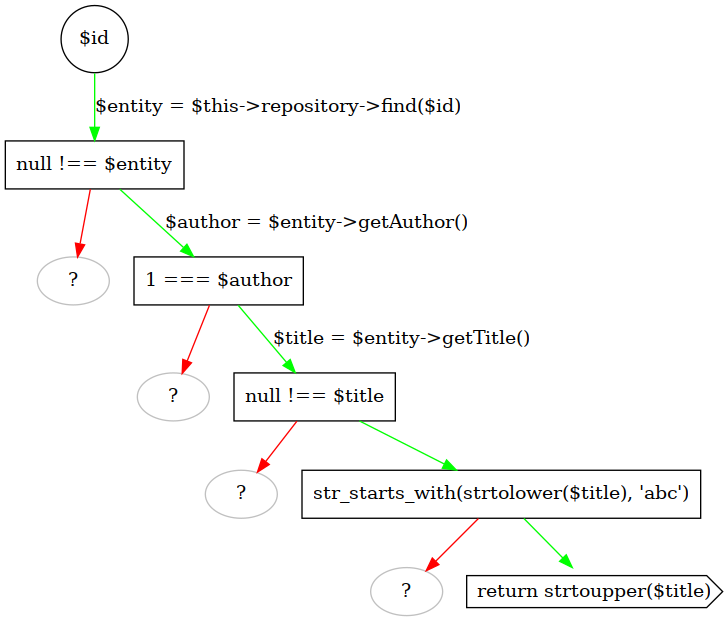
\includegraphics[height=.70\paperheight]{src/session/complexity/resources/complexity-example.png}}

    \note[item]{
        The green color represent the happy path, the red one the unhappy path.
    }
    \note[item]{
        Notice here the interogation marks, we'll come back to it later on.
    }
    \note[item]{
        Have you ever asked yourself why sometimes we have to compare a value
        against null ? We will come back to this later.
    }
\end{frame}

\begin{frame}[fragile,c]
    \frametitle{Complexity}
    \framesubtitle{Cyclomatic complexity}

    Conditions and type checks adds complexity to a program, we are going to see
    how we can get rid of them in a nice an clean way.

    \note[item]{
        FYI, The controversial value "null" is a billion dollar mistake
        according to its creator Tony Hoare, the creator of the quicksort algo,
        the null value and ALGOL. In a software conference in 2009, he
        apologized for inventing the null reference!
    }
    \note[item]{
        But let's come back to our subject, how could we get rid of these
        conditions in our snippet... we will come back to the the null value
        later.
    }
\end{frame}

\begin{frame}[fragile,c]
    \Large
    But\pause\ but\pause\ but\pause ... we need conditions !

    \note[item]{
        Of course we need conditions, this is the basically what defines the
        logic. What I mean here, is how could we reduce the way we write our
        code so it contains less conditions while being easy to read and hack.
    }
\end{frame}

\begin{frame}[fragile,c]
    \frametitle{Complexity}
    \framesubtitle{Reducing the amount of nested conditions}
    \Huge
    EARLY RETURNS !

    \note[item]{
        Boom ! That's one way to do it.
    }
    \note[item]{
        For those who works with me, they already know what I'm talking about,
        I'm always hammering people to use and abuse them. But why ?
    }
    \note[item]{
        Early returns allows you to have a clearer view of what you're trying
        to do by ``flattening'' the structure of the code using ``early returns''
        statements. Let's have a look at an example.
    }
\end{frame}

\begin{frame}[fragile,c]
    \frametitle{Complexity}
    \framesubtitle{Cyclomatic complexity}

    \begin{lstlisting}[language=php]
    if ($expr1 && $expr2 && $expr3) {
        return true;
    }

    return false;
    \end{lstlisting}

    \pause

    is equivalent to:

    \begin{lstlisting}[language=php]
    if (! $expr1) {
        return false;
    }

    if (! $expr2) {
        return false;
    }

    if (! $expr3) {
        return false;
    }

    return true;
    \end{lstlisting}

    \note[item]{
        I guess you already had such pattern in your code right?
        The relevant part of the code or the happy path is wrapped in a huge
        condition expression, or even worst. And then, the last line of your
        function is the unhappy path. I don't like that. It's not straighforward
        when skimming the code to find what you're looking for or to find what
        is the return value of an algorithm.
    }
    \note[item]{
        Using early returns let you to split the huge condition expression
        into multiple small conditions.
    }
    \note[item]{
        Those early returns are inverted so we can bail out as soon as we
        encounter something wrong.
    }
    \note[item]{
        Notice also that the happy path is usually after all these ``guards''.
    }
    \note[item]{
        Usually, by looking at the last line of a function, method or algorithm,
        you know what it is returning in case of successful execution.
    }
    \note[item]{
        It is often easier to understand than having a huge logical expression
        to evaluate.
    }
    \note[item]{
        Let you customize a precise custom error value per condition.
    }
    \note[item]{
        Let's apply this trick to our Symfony snippet now...
    }
\end{frame}

\begin{frame}
    \frametitle{Complexity}
    \framesubtitle{Cyclomatic complexity}

    \lstinputlisting{src/session/complexity/resources/complexity-example-early-returns.php}
\end{frame}

\begin{frame}
    \frametitle{Complexity}
    \framesubtitle{Cyclomatic complexity}

    \begin{itemize}[<+->]
        \item Think to the ``\textcolor{red}{unhappy}'' paths at first
        \item The ``\textcolor{green}{happy}'' path, is usually the last line,
        \item Easier to read, understand,
        \item Longer to write.
    \end{itemize}
\end{frame}

\begin{frame}[fragile,c]
    \frametitle{Complexity}
    \framesubtitle{Cyclomatic complexity}
    \Huge
    Programming paradigms

    \note[item]{
        This one is a bit funny but...
    }
    \note[item]{
        Another way to reduce the complexity of your code is to reduce the
        amount of code you write. Obviously.
    }
    \note[item]{
        Indeed. Some paradigms make your code more verbose and much prone to
        issues by creating unecessary variables and statements.
    }
\end{frame}

\begin{frame}
    \frametitle{Complexity}
    \framesubtitle{Imperative programming}

    Imperative programming tells the machine how to do something.

    \pause

    (resulting in what you want to happen).
\end{frame}

\begin{frame}
    \frametitle{Complexity}
    \framesubtitle{Declarative programming}

    Declarative programming tells the machine what you would like to happen.

    \pause

    (and the computer figures out how to do it)
\end{frame}

\begin{frame}
    \frametitle{Complexity}
    \framesubtitle{Imperative and declarative programming}

\lstinputlisting[caption={Imperative programming}]{src/session/history/resources/oop.js}
\pause
\lstinputlisting[caption={Declarative programming}]{src/session/history/resources/fp.js}
\end{frame}

\begin{frame}
    \frametitle{Complexity}
    \framesubtitle{Imperative and declarative programming}

\lstinputlisting[caption={Imperative programming}]{src/session/complexity/resources/imperative1.js}
\pause
\lstinputlisting[caption={Declarative programming}]{src/session/complexity/resources/declarative1.js}
\end{frame}

\begin{frame}
    \frametitle{Complexity}
    \framesubtitle{Abstracting away the complexity?}

    Have you every wondered why there are so much packages existing for a
    particular languages?\\
    \pause
    Most probably they were created to fix particular and recurrent issues or
    boring problematic?\\
    \pause
    Sometimes it could be nice to query the language package managers to find if
    the solution to your problem doesn't already exists!\\
    \pause
    This would delegate the responsibility somewhere else and reduce the overall
    complexity of your application.\\
    \pause
    It is also less code to maintain and thus, less prone to bugs.
\end{frame}

\begin{frame}
    \frametitle{Complexity}
    \framesubtitle{Confidence in other packages?}

    Relying on someone else's code means a lot, for some reason people prefer
    redoing things on their own.\\
    \pause
    I believe that developers should be able to evaluate the trust into a
    package based on some key indicators.\\
    \pause
    Tests, popularity, code lisibility, code extensibility, code practices...
\end{frame}

\begin{frame}
    \frametitle{Complexity}
    \framesubtitle{Confidence in other packages?}

    This is the reason why when making a package, it's better to be as strict
    as possible so the developer using your code doesn't have any surprise when
    using your code in its own.\\
    \pause
    Avoid mixing types, throw proper exceptions in case of issues, etc etc.\\
    \pause
    Let's remind to the audience how to put those tips in practice.
\end{frame}
